%!TEX TS-program = xelatex
\documentclass[a4paper, 12pt]{article}
\usepackage{barinovxesimple}
\geometry{top=25mm}
\geometry{bottom=35mm}
\geometry{left=35mm}
\geometry{right=20mm}
\setlist{labelindent=\parindent,leftmargin=*}
\begin{document}
\thispagestyle{empty}
\begin{center}
    \textit{Федеральное государственное автономное образовательное\\ учреждение высшего образования }

    \vspace{0.5ex}

        \textbf{«Московский физико-технический институт\\ (национальный исследовательский университет)»}
\end{center}

\vspace{10ex}

\begin{center}
    \vspace{13ex}

    \so{\textbf{Лабораторная работа №_._._}}

    \vspace{1ex}

    по курсу общей физики

    на тему:

    \textbf{\textit{<<>>}}

    \vspace{30ex}

    \begin{flushright}
        \noindent
        \textit{Работу выполнил:}\\  
        \textit{Баринов Леонид \\(группа Б02-827)}
    \end{flushright}
    \vfill
    Долгопрудный \\2019
\newpage
\setcounter{page}{1}
\fancyhead[R]{\nouppercase{\leftmark}}	
\end{center}

\section{Аннотация}
В работе будет измерена энергия первого уровня атома гелия в
динамическом и статическом режимах методом электронного возбуждения.





\section{Теоретические сведения}
В квантовой механике энергия, которой может обладать частица,
находящаяся в потенциальной яме в связанном состоянии, принимает
дискретные значения, причем наинизший (основной) уровень лежит выше
дна ямы. 

Исходя из соотношения неопределенности $\Delta p \Delta x \simeq
\hbar$ легко оценить энергию основного состояния частицы в
прямоугольной яме шириной $a$ с бесконечными стенками. В данном случае
$\Delta x \simeq a$, а потому импульс частицы $p = \Delta p \simeq
\hbar/ a$. Если отсчитывать энергию частицы от дна ямы, то минимальная
энергия будет равна
\begin{equation}
    E = \frac{p^2}{2m} \simeq \frac{\hbar^2}{2 m a^2}
    \label{eq:1}
\end{equation}

Разность между энергией основного состояния квантово-механической
системы и энергией, соответствующей минимуму потенциальной энергии,
называется \emph{нулевой энергией}. 

Чтобы найти возможные (разрешенные) уровни энергии частицы в заданном
потенциале, надо решить стационарное уравнение Шредингера, которое в
одномерном случае имеет вид
\begin{equation}
    - \frac{\hbar^2}{2m} \frac{d^2 \psi}{dx^2} + U(x)\psi = E \psi
    \label{eq:2}
\end{equation}

Физический смысл имеют лишь конечные, однозначные, непрерывные и
гладкие решения этого уравнения. В соответствии с граничными условиями
в одномерной потенциальной яме с бесконечными стенками возможные
уровни энергии частицы определяются соотношением
\begin{equation}
    E_n = \frac{\pi^2 \hbar^2}{2ma^2} n^2, \quad n =1,2,3,\ldots
    \label{eq:3}
\end{equation}

Частица, <<запертая>> в потенциальной яме, может иметь только
дискретные (квантовые) значения энергии, которые называются уровнями
энергии частицы в заданном потенциале.

Если частица находится в прямоугольной потенциальной яме с одной из
стенок конечной высоты $U_0$, то минимальное значение ее энергии
(нулевая энергия) равно
\begin{equation}
    E = \frac{\pi^2 \hbar^2}{8ma^2}
    \label{eq:4}
\end{equation}

Стационарные уровни в такой яме возникают лишь в том случае, если $E <
U_0$, т.е. при условии
\begin{equation}
    U_0 a^2 > \frac{\pi^2 \hbar^2}{8m}
    \label{eq:5}
\end{equation}

В левой части этого неравенства стоят параметры потенциальной ямы, а в
правой --- только масса частицы и универсальные константы. Если
полученное нами условие не выполнено, в ней не помещается ни одного
энергетического уровня.

Вот в одно- и двумерной ямах (в которых поле есть функция только от
одной или двух координат) всегда имеются уровни отрицательной энергии,
т.е. даже при условии
\begin{equation}
    |U| \ll \frac{\hbar^2}{ma^2}
    \label{eq:6}
\end{equation}

Так, например, в сколь угодной мелкой одномерной яме шириной $a$ и
глубиной $U$ энергия связанного состояния равна
\begin{equation}
    E = \frac{mU^2a^2}{2 \hbar^2} \ll U
    \label{eq:7}
\end{equation}

Согласно квантовой механике частица, находящаяся в потенциальной яме
со <<стенками>> конечной толщины, в результате туннельного эффекта
может покинуть потенциальную яму даже в том случае, если ее энергия
меньше высоты стенок потенциальной ямы. В таком случае, что уровни
энергии частицы являются \emph{квазистационарными}, так как частица
<<живет>> в таком состоянии конечное время. О таких уровнях также
говорят как о \emph{метастабильных}. Все уровни частицы в потенциале со
стенками конечной толщины имеют конечную ширину, зависящую,
естественно, от энергии состоянии и формы потенциала.

Дискретность энергетических уровней микрочастицы, находящейся в
потенциальной яме, отчетливо проявляется в спектрах излучения и
поглощения атомов, молекул, ядер. Ярким подтверждением дискретности
атомных уровней являются эксперименты по возбуждению и ионизации
атомов электронном ударов, впервые проведенные в 1913г. Д.Франком и
Г.Герцем. 




\section{Оборудование}
Одним из простых опытов, подтверждающих существование дискретных
уровней энергии атомов, является эксперимент, известный под названием
опыта Франка и Герца. Схема опыта изображена на \fig{fig:1}. 

Разреженный одноатомный газ (в нашем случае гелий) заполняет
трехэлектродную лампу. Электроны, испускаемые разогретым катодом.
ускоряются в постоянном электрическом поле, созданном между катодом и
сетчатым анодом лампы. Передвигаясь от катода к аноду, электроны
сталкиваются с атомами гелия. Если энергия электрона, налетающего на
атом, недостаточна для того, чтобы перевести его в возбужденное
состояние (или ионизовать), то возможны только упругие соударения, при
которых электроны почти не теряют энергии, так как их масса в тысячи
раз меньше массы атомов.

По мере увеличения разности потенциалов между анодом и катодом энергия
электронов увеличивается и, в конце концов, оказывается достаточной
для возбуждения атомов. При таких неупругих столкновениях кинетическая
энергия налетающего электрона передается одному из атомных электронов,
вызывая его переход на свободный энергетический уровень (возбуждение)
или совсем отрывая его от атома (ионизация).

\begin{figure}[H]
    \floatsetup{heightadjust=object,valign=c}
    \begin{floatrow}

        \ffigbox{
        \caption{Схема опыта Франка и Герца}
        \label{fig:1}
    }
        {
        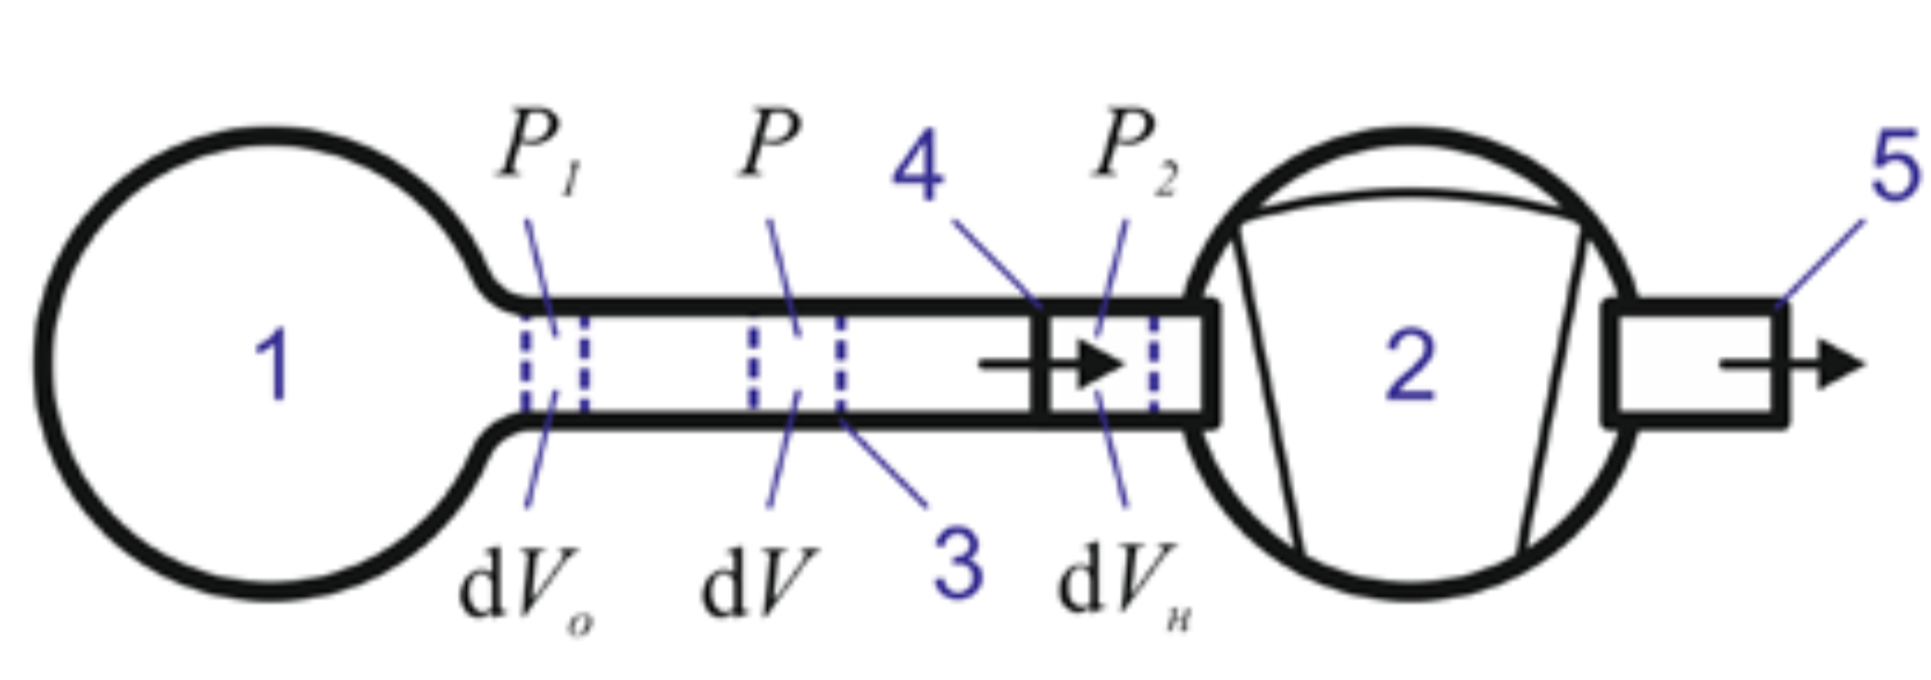
\includegraphics[width=\linewidth]{1}
    }

        \ffigbox{
        \caption{Схематический вид зависимости тока коллектора от
        напряжения на аноде}
        \label{fig:2}
    }
        {
        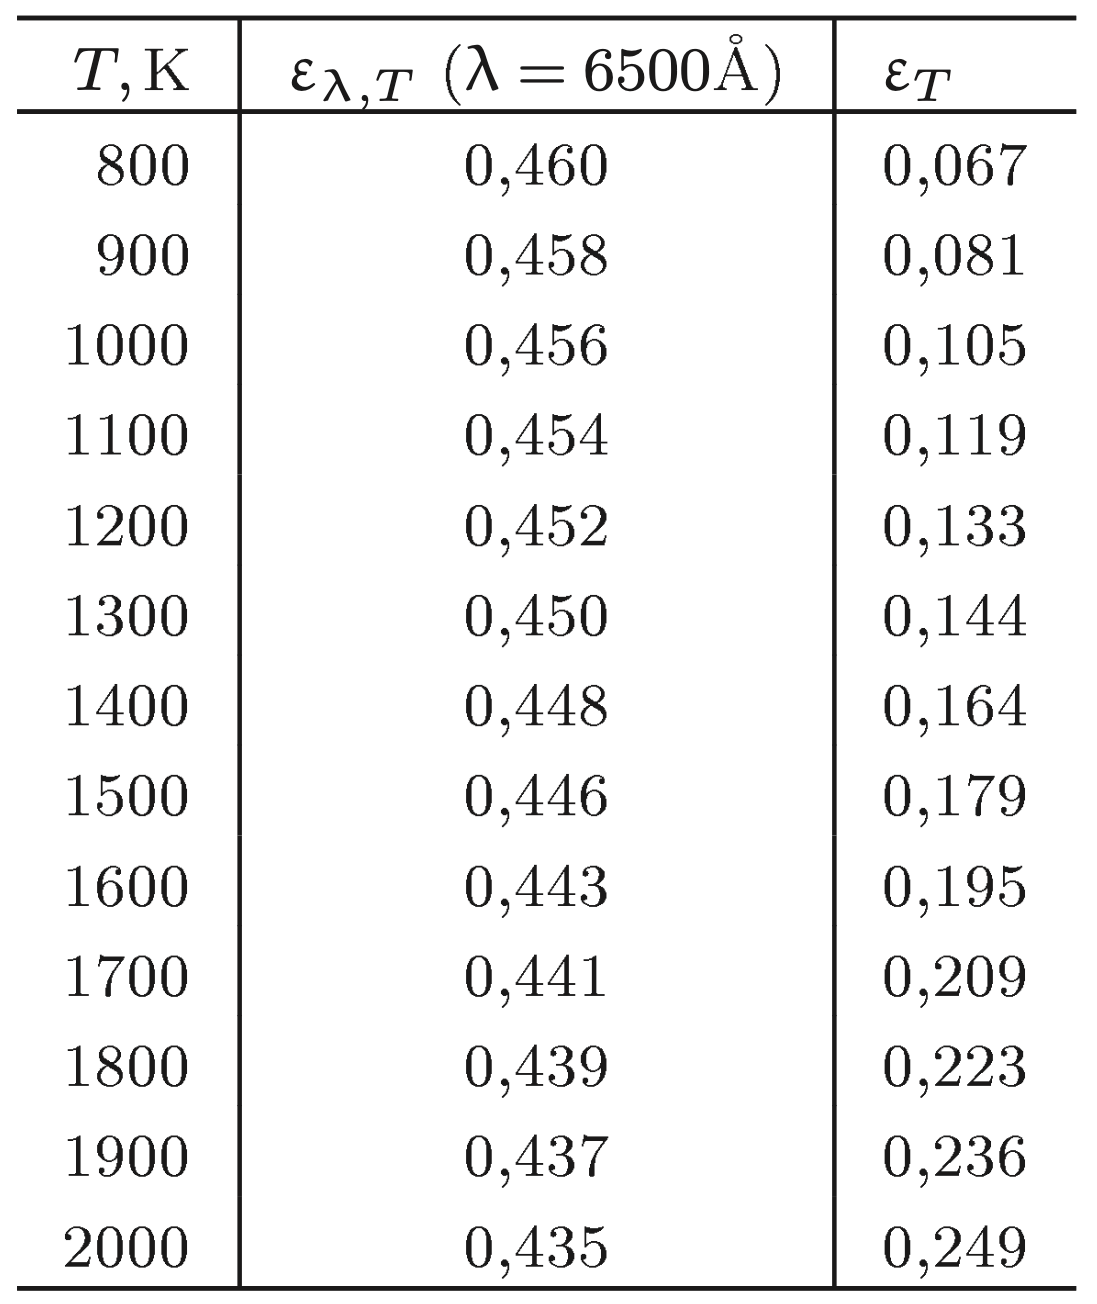
\includegraphics[width=0.9\linewidth]{2}
    }
    \end{floatrow}
\end{figure}




Третьим электродом лампы является коллектор. Между ним и анодом
поддерживается небольшое задерживающее напряжение (потенциал
коллектора меньше потенциала анода). Ток коллектора, пропорциональный
числу электронов, попадающих на него за секунду, измеряется микроамперметром.

При увеличении потенциала анода ток в лампе вначале растет, подобно
тому как это происходит в вакуумном диоде \ffig{fig:2}. Однако, когда
энергия электронов становится достаточной для возбуждения атомов, ток
коллектора резко уменьшается. Это происходит потому, что при неупругих
соударениях с атомами электроны почти полностью теряют свою энергию и
не могут преодолеть задерживающего потенциала (около 1 В) между анодом
и коллектором. При дальнейшем увеличении потенциала анода ток
коллектора вновь возрастает: электроны, испытавшие неупругие
соударения, при дальнейшем движении к аноду успевают набрать энергию,
достаточную для преодоления задерживающего потенциала.

Следующее замедление роста тока происходит в момент, когда часть
электронов неупруго сталкивается с атомами два раза: первый раз
посередине пути, второй у анода и т. д. Таким образом, на кривой
зависимости тока коллектора от напряжения анода имеется ряд максимумов
и минимумов, отстоящих друг от друга на равные расстояния $\Delta V$; эти
расстояния равны энергии первого возбужденного состояния.

При тщательной постановке опыта можно увидеть и тонкую структуру
кривой спада тока, содержащую ряд минимумов, соответствующих
возбуждению других уровней и ионизации атома гелия. Для этого нужны
лампы специальной конструкции. В нашей постановке опыта эта тонкая
структура не видна.

\subsection{Экспериментальная установка}
Схема экспериментальной установки изображена на \ffig{fig:3}. Для опыта
используется серийная лампа ионизационного манометра ЛМ-2, 
заполненная гелием до давления $\simeq 1\ \text{Тор}$.

\begin{figure}[H]
    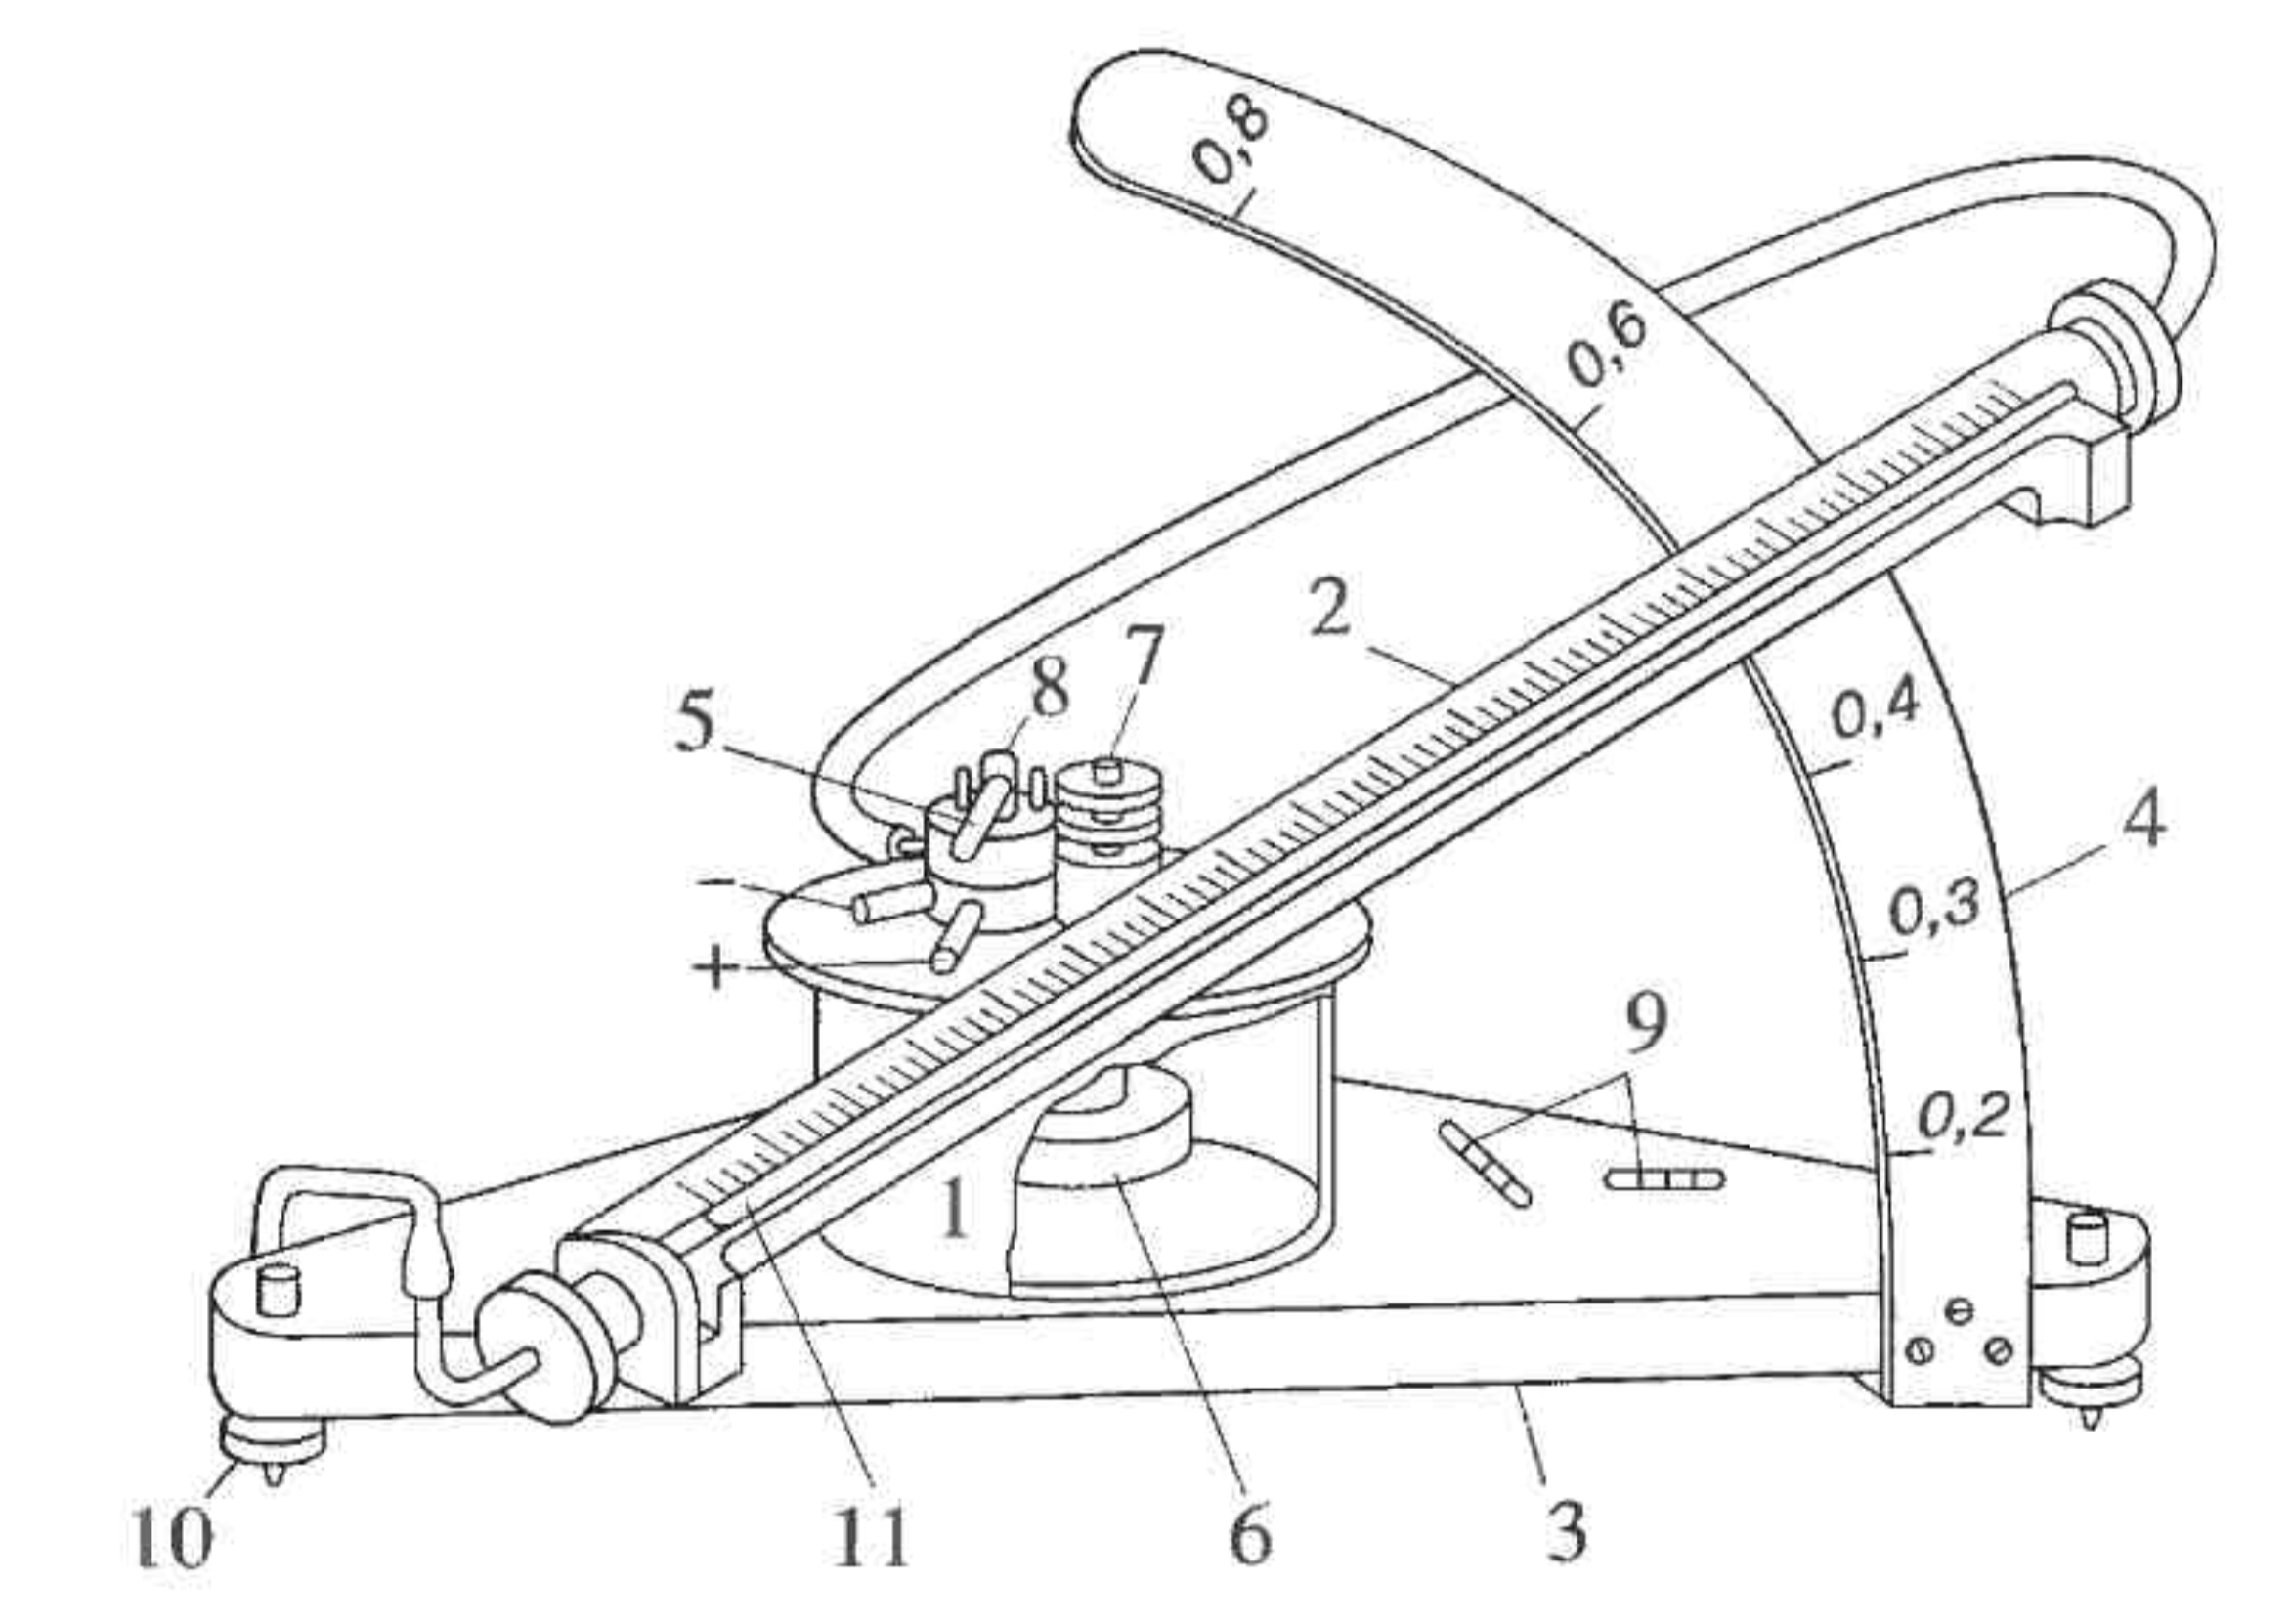
\includegraphics[width=0.65\linewidth]{3} 
    \caption{Схема экспериментальной установки}
    \label{fig:3}
\end{figure}

Источником
электронов является вольфрамовый катод, нагреваемый переменным током.
Напряжение накала подается от стабилизированного источника питания
С. Ток накала контролируется амперметром А.

В качестве анода используется двойная спираль, окружающая катод. Роль
коллектора играет полый металлический цилиндр, соосный с катодом и
анодом.

Ускоряющее напряжение подается на анод от выпрямителя B. Величина
этого напряжения регулируется потенциометром $\text{П}_{3}$ и измеряется
вольтметром $V_1$. 


Источник задерживающего потенциала — батарея 
4,5 \text{В}; величина напряжения регулируется 
потенциометром $\text{П}_{2}$ и измеряется вольтметром $V_2$. Ток в
цепи коллектора
регистрируется микроамперметром.

Схему можно переключать из статического режима измерений в
динамический режим с помощью ключа $K_3$. На \fig{fig:3} две части сдвоенного
ключа $K_3$ изображены отдельно. При динамическом режиме работы
ускоряющий потенциал подается с понижающего трансформатора $T$ (220/50
$\text{В}$), а ток коллектора регистрируется осциллографом,
подключенным к нагрузочному резистору $R$. 

При определении энергии электронов по разности потенциалов между
анодом и катодом следует иметь в виду, что из-за контактной разности
потенциалов между катодом и анодом первый максимум но соответствует
потенциалу первого возбужденного уровня. Однако контактная разность
потенциалов так сдвигает все максимумы, что расстояние между ними не
меняется.

Схема экспериментальной установки, изображенной на \fig{fig:3}, в
нашей работе конструктивно осуществлена следующим образом. Наполненная
гелием лампа ЛМ-2 расположена непосредственно на корпусе блока
источников питания (БИП). Напряжение к электродам лампы подводится от
источников питания, находящихся в корпусе прибора. Регулировка
напряжения и выбор режима работы производятся при помощи ручек
управления, выведенных на лицевую панель БИП \ffig{fig:4}. Включение
всех источников питания осуществляется включением БИП в сеть.

В статическом режиме напряжение $V_\text{a}$ между анодом и катодом
измеряется цифровым вольтметром В7-22А, подключенным к клеммам
<<Вольтметр>> прибора. Ток коллектора $I_\text{к}$ измеряется
микроамперметром, вся шкала которого соответствует току $100\
\text{мкА}$.


\begin{figure}[H]
    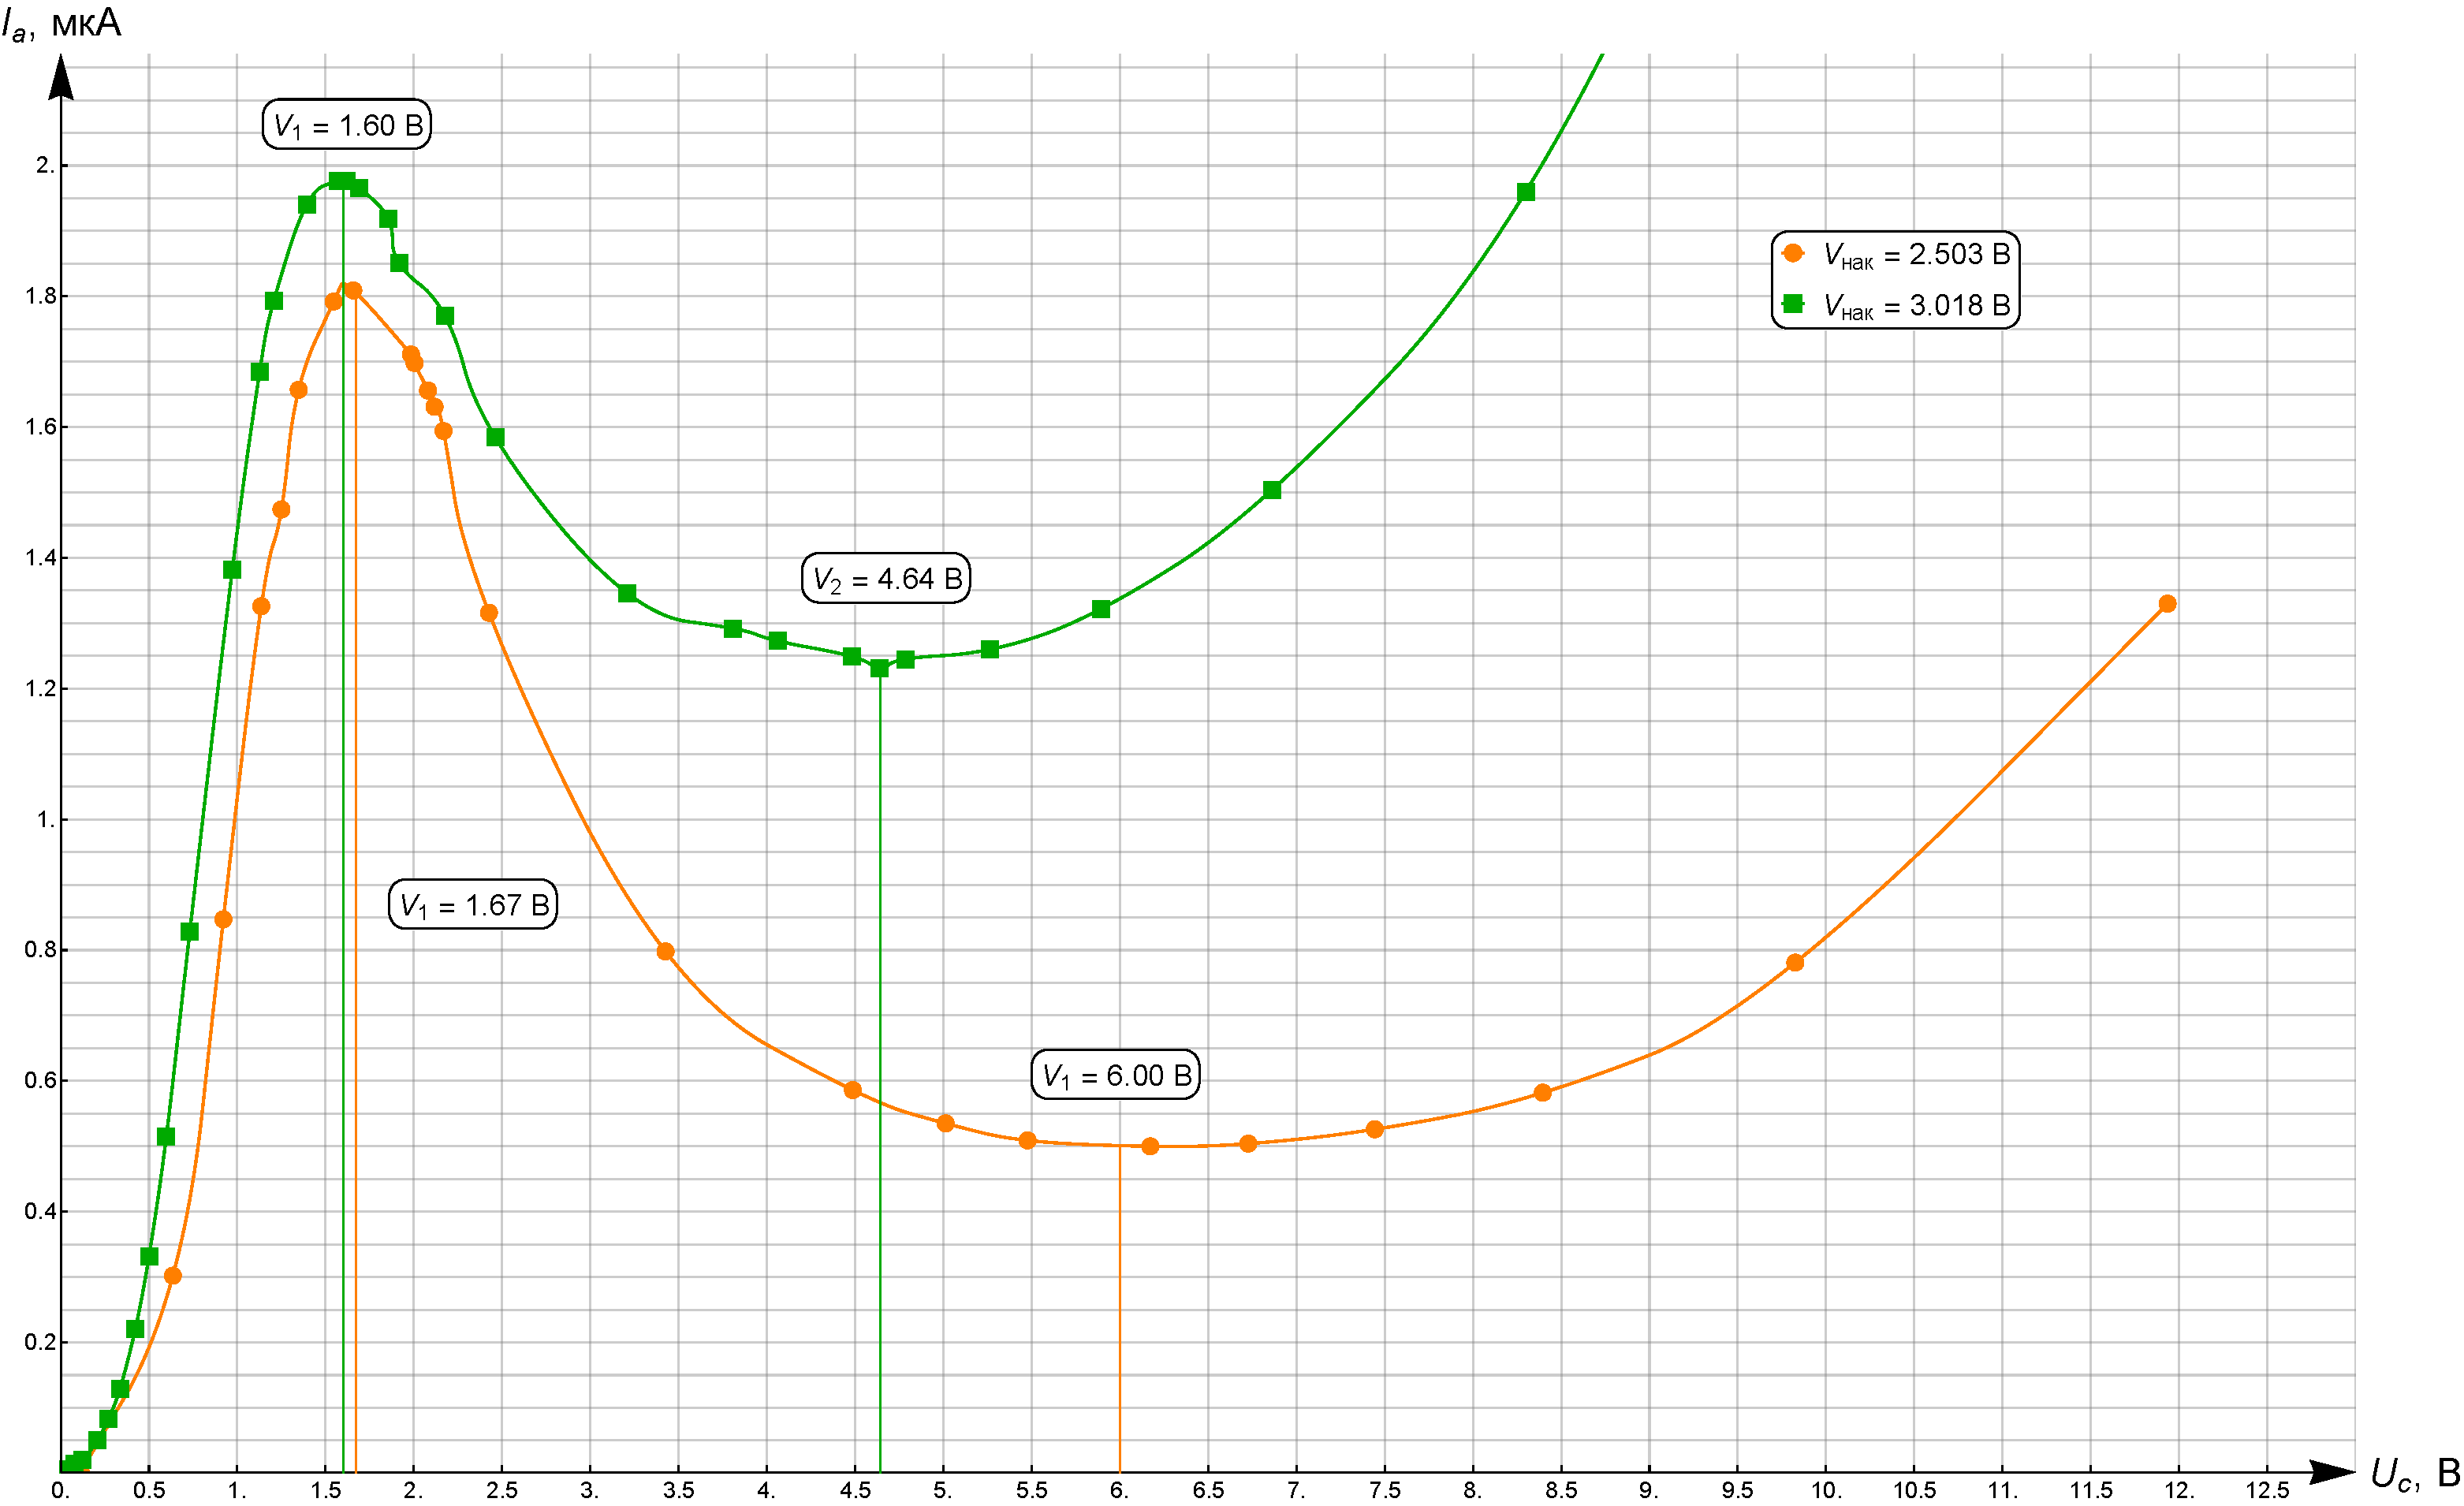
\includegraphics[width=\linewidth]{10} 
    \caption{Блок-схема экспериментальной установки}
    \label{fig:4}
\end{figure}





\section{Результаты измерений и обработка результатов}

Ключом $K_3$ переведем схему в динамический режим измерений. Проведем
наблюдение для вольт-амперной характеристики $I_\text{к} =
I_\text{к}(V_\text{а})$ лампы.


\begin{figure}[H]
    \floatsetup{heightadjust=object,valign=c}
    \begin{floatrow}

        \ffigbox{
        \caption{$V_2 = 4\ \text{В}$}
    }
        {
        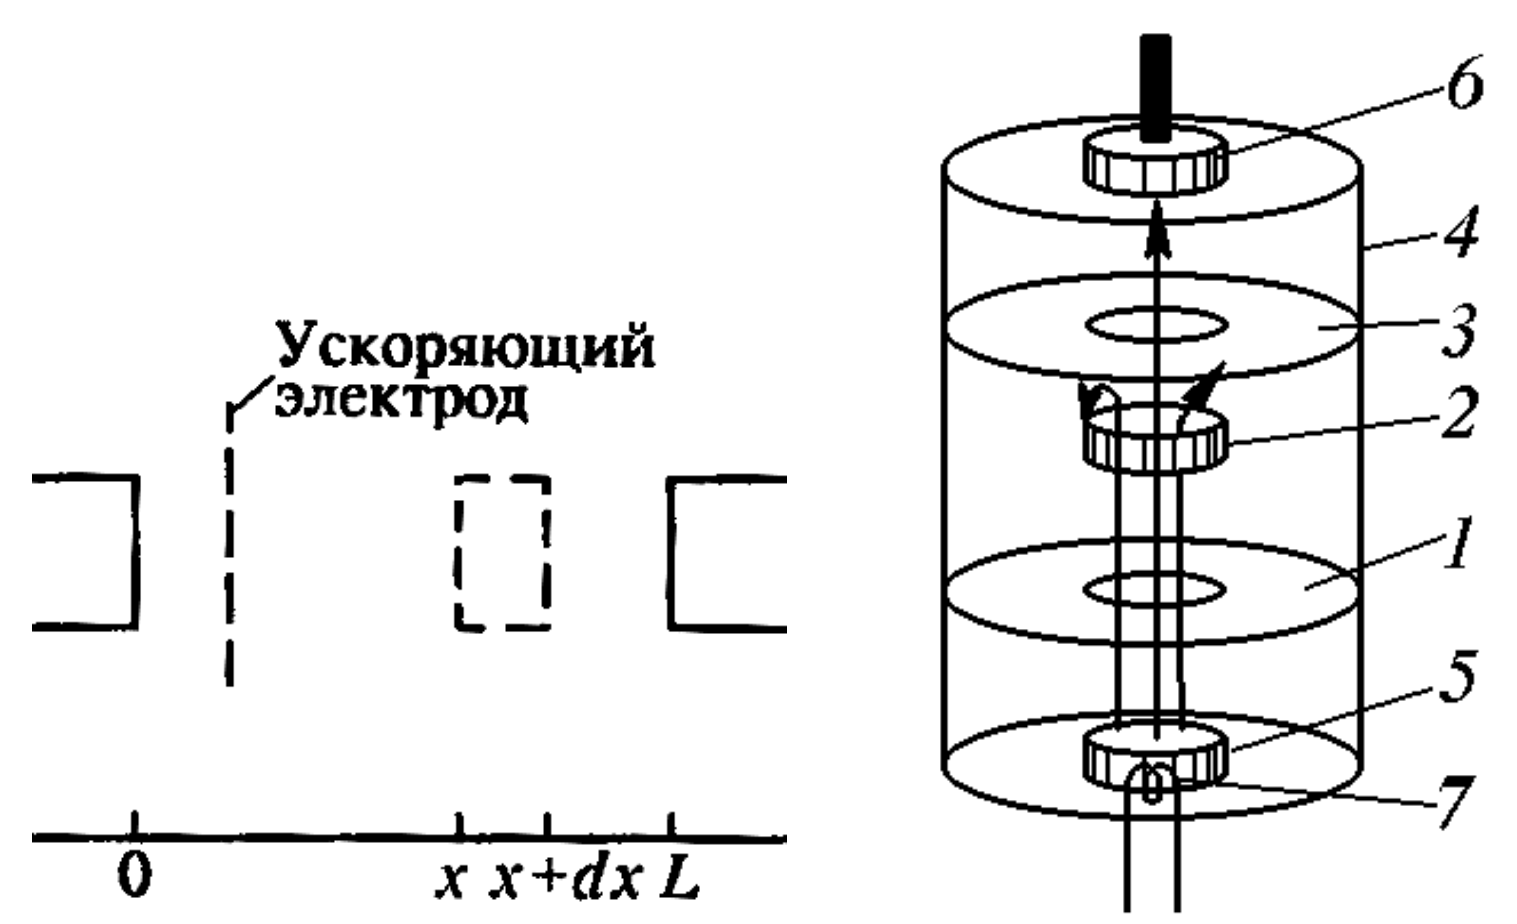
\includegraphics[width=0.8\linewidth]{4}
    }

        \ffigbox{
        \caption{$V_2 = 4\ \text{В}$}
    }
        {
        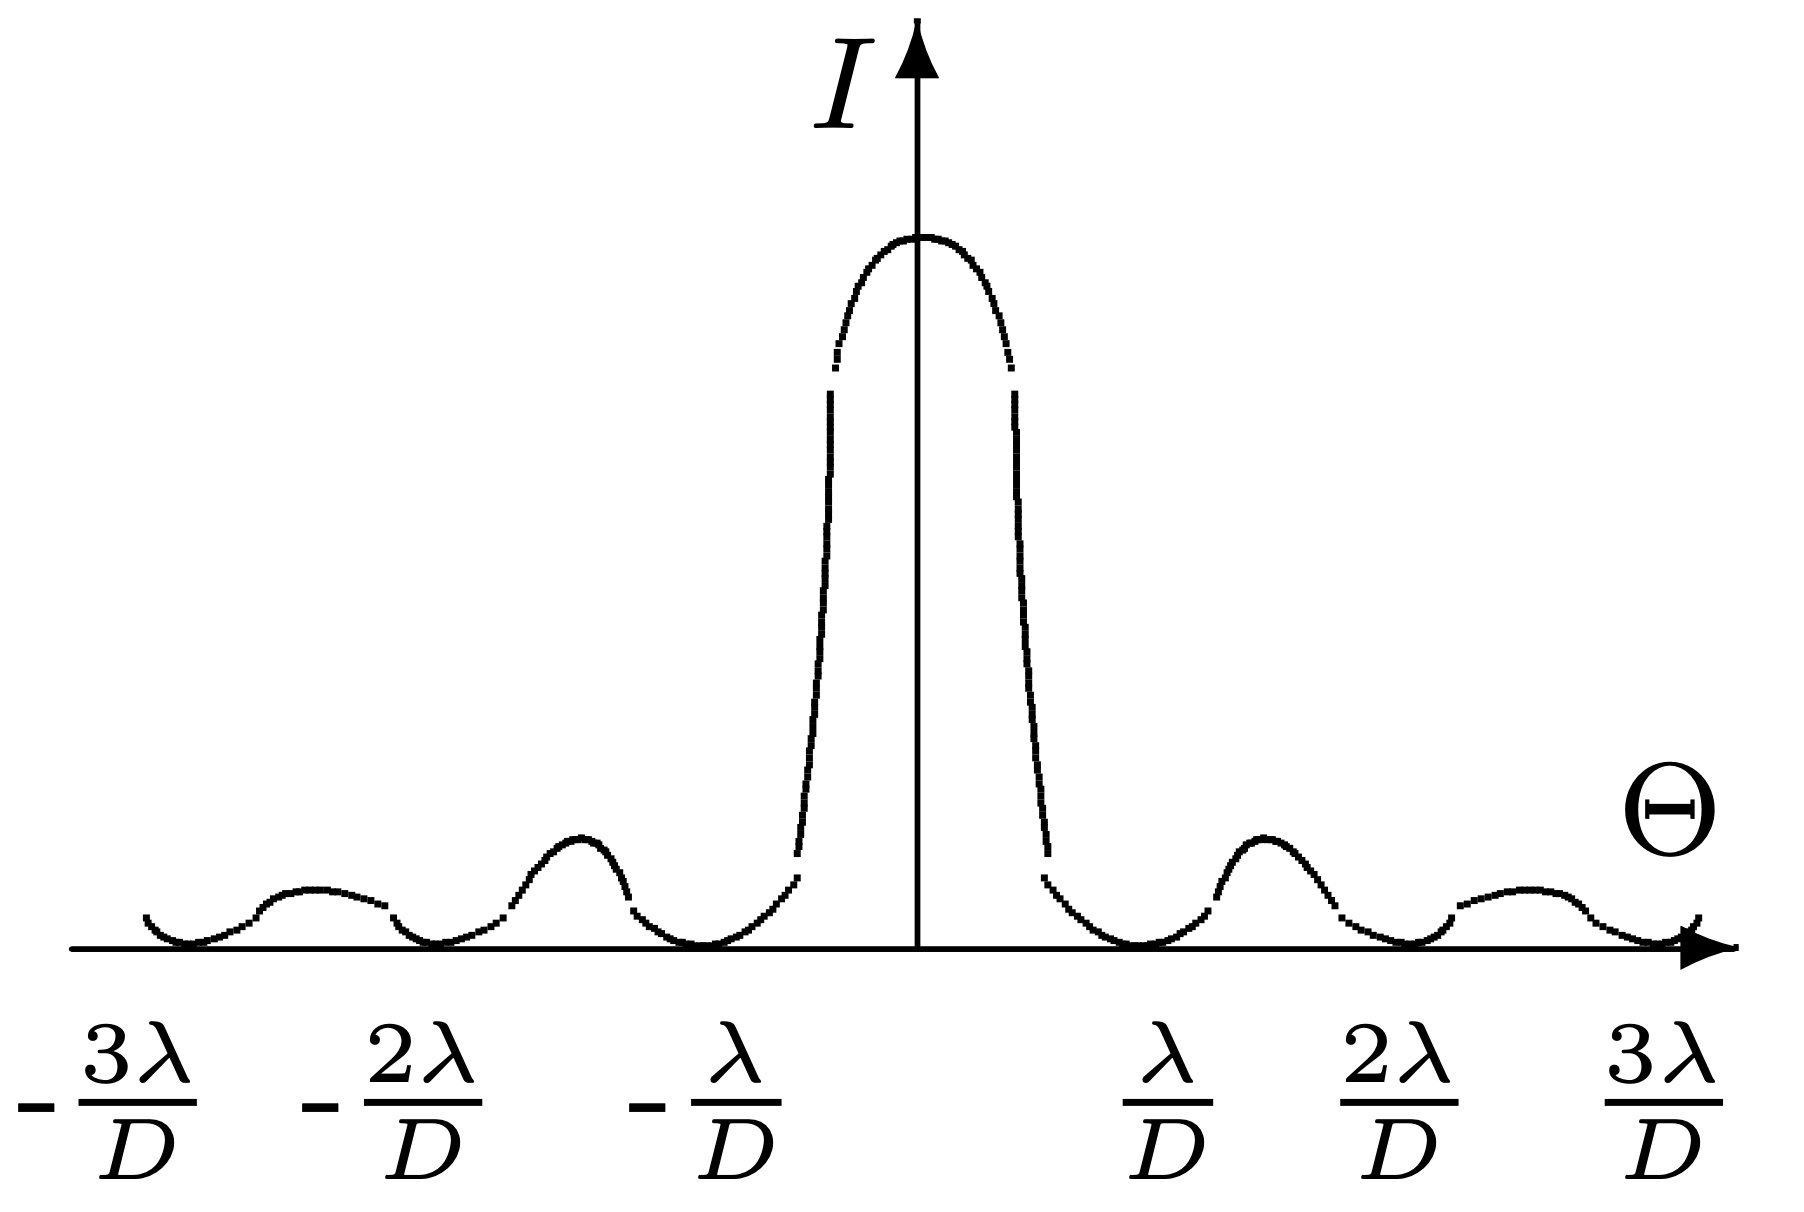
\includegraphics[width=0.8\linewidth]{5}
    }
    \end{floatrow}
\end{figure}

По расстоянию между соседними максимумами на осциллограммах определим
энергию возбуждения первого уровня атома гелия. Одно маленькое деление
соответствует $1\ \text{В}$. Усредняя получим:
\[
    E_1^\text{дин} = (25,0 \pm 0,8)\ \text{эВ}
\]

Получим вольт-амперную характеристику $I_\text{к} = f (V_\text{а})$ в
статическом режиме измерений \ffig{fig:11}.


\begin{figure}[H]
    \floatsetup{heightadjust=object,valign=c}
    \begin{floatrow}

        \ffigbox{
        \caption{$V_2 = 6\ \text{В}$}
    }
        {
        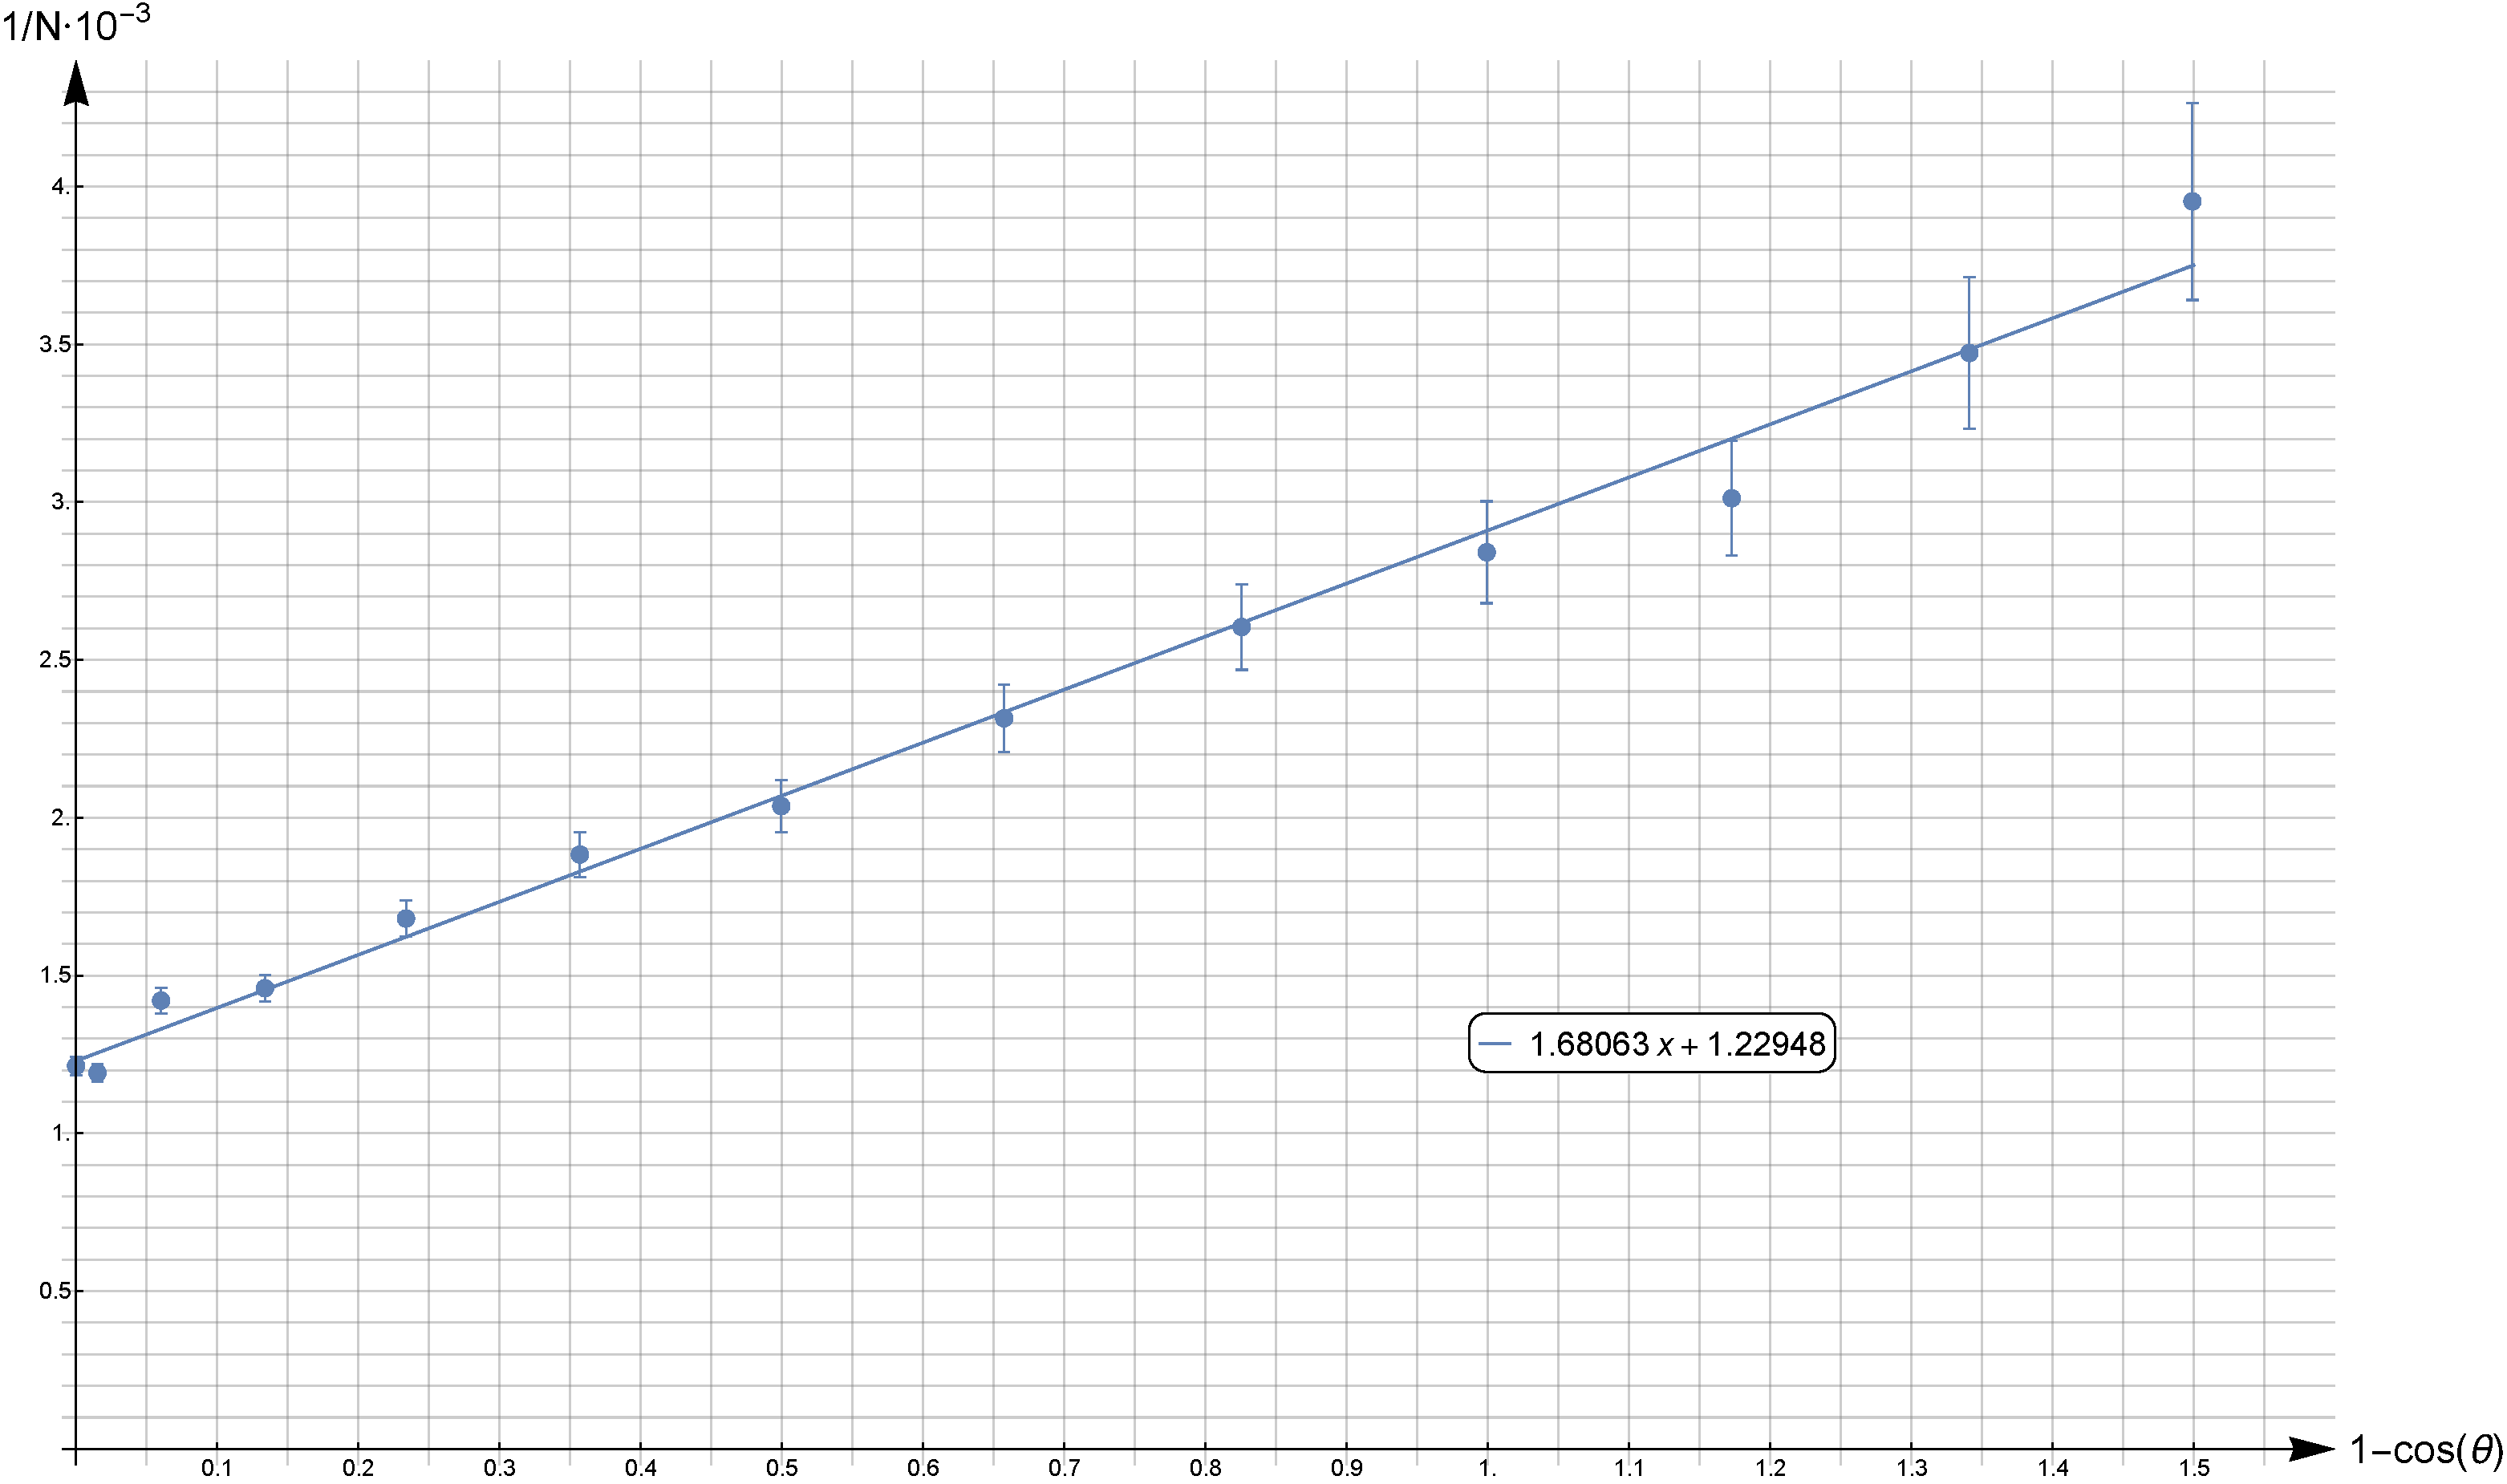
\includegraphics[width=0.8\linewidth]{6}
    }

        \ffigbox{
        \caption{$V_2 = 6\ \text{В}$}
    }
        {
        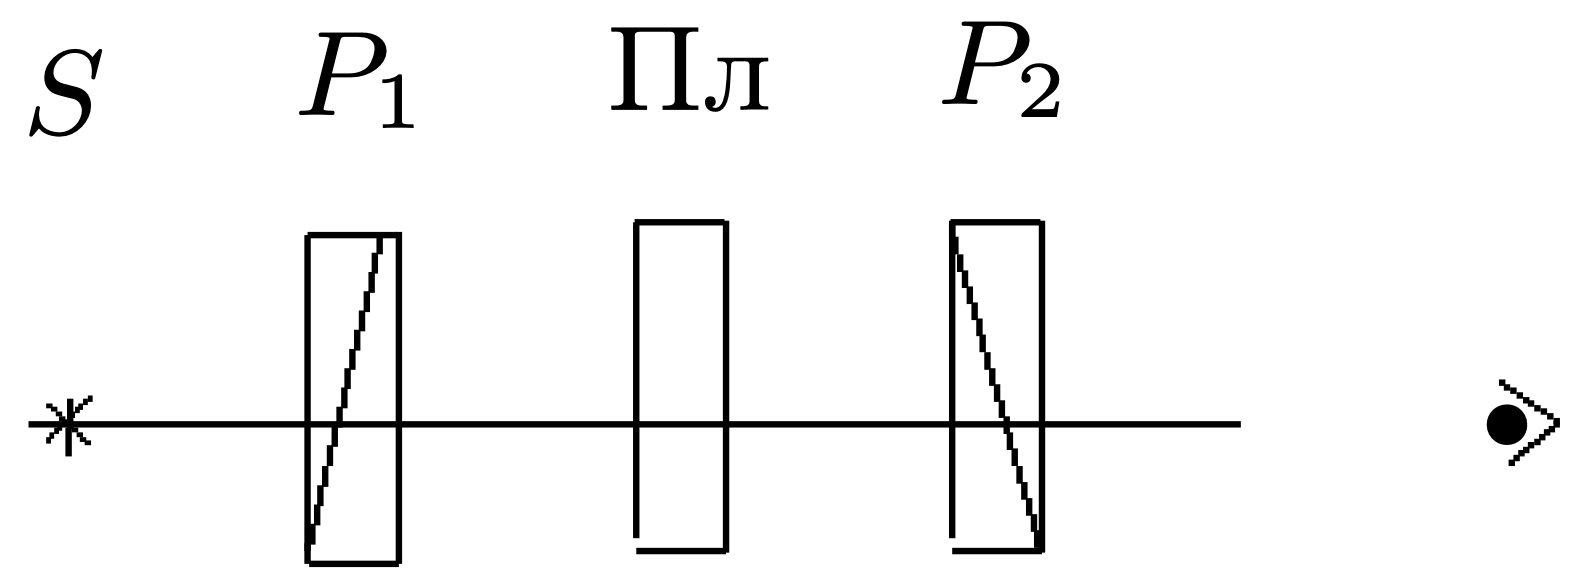
\includegraphics[width=0.8\linewidth]{7}
    }
    \end{floatrow}
\end{figure}


\begin{figure}[H]
    \floatsetup{heightadjust=object,valign=c}
    \begin{floatrow}

        \ffigbox{
        \caption{$V_2 = 8\ \text{В}$}
    }
        {
        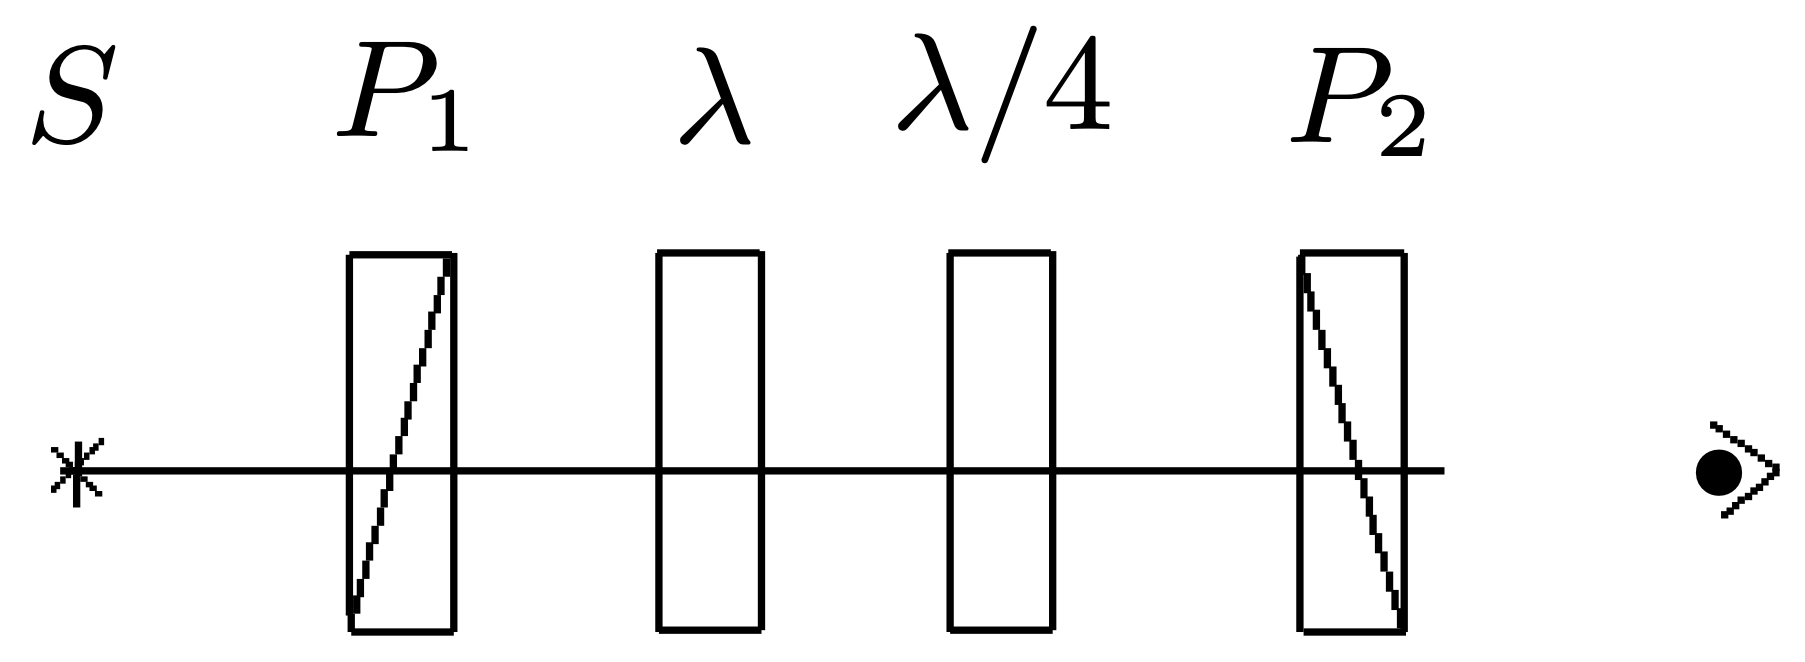
\includegraphics[width=0.8\linewidth]{8}
    }

        \ffigbox{
        \caption{$V_2 = 8\ \text{В}$}
    }
        {
        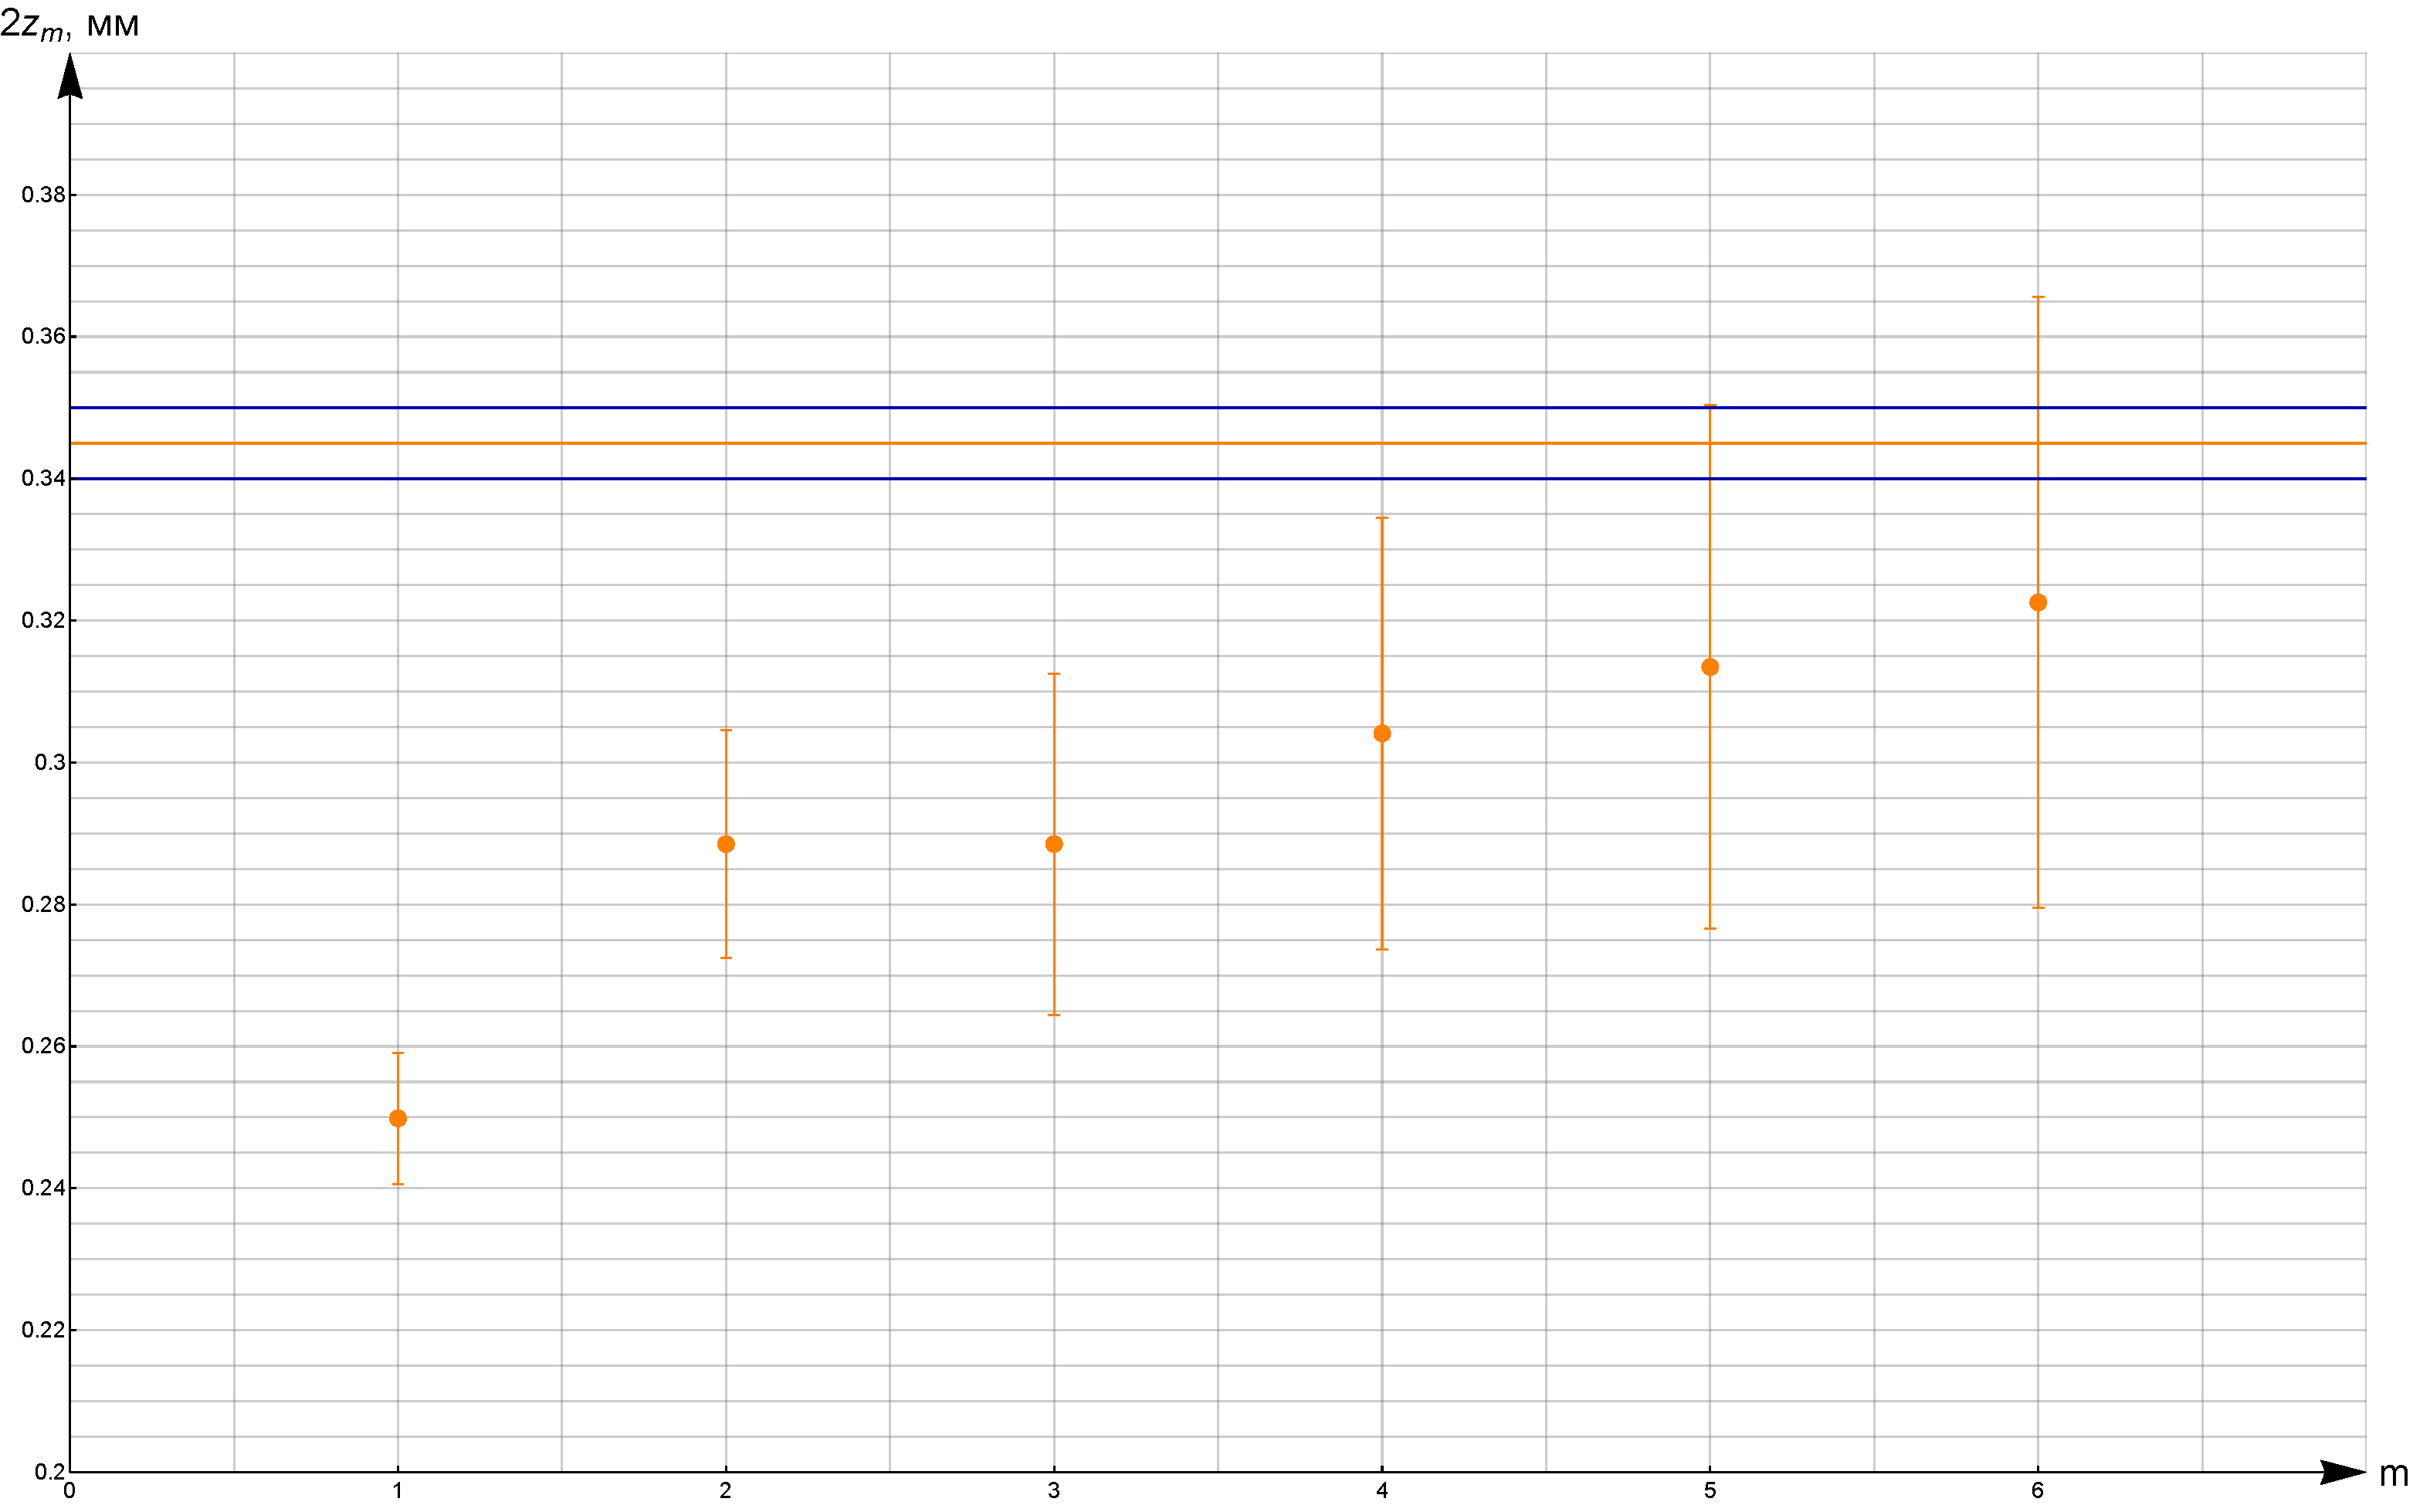
\includegraphics[width=0.8\linewidth]{9}
    }
    \end{floatrow}
\end{figure}



\begin{figure}[H]
    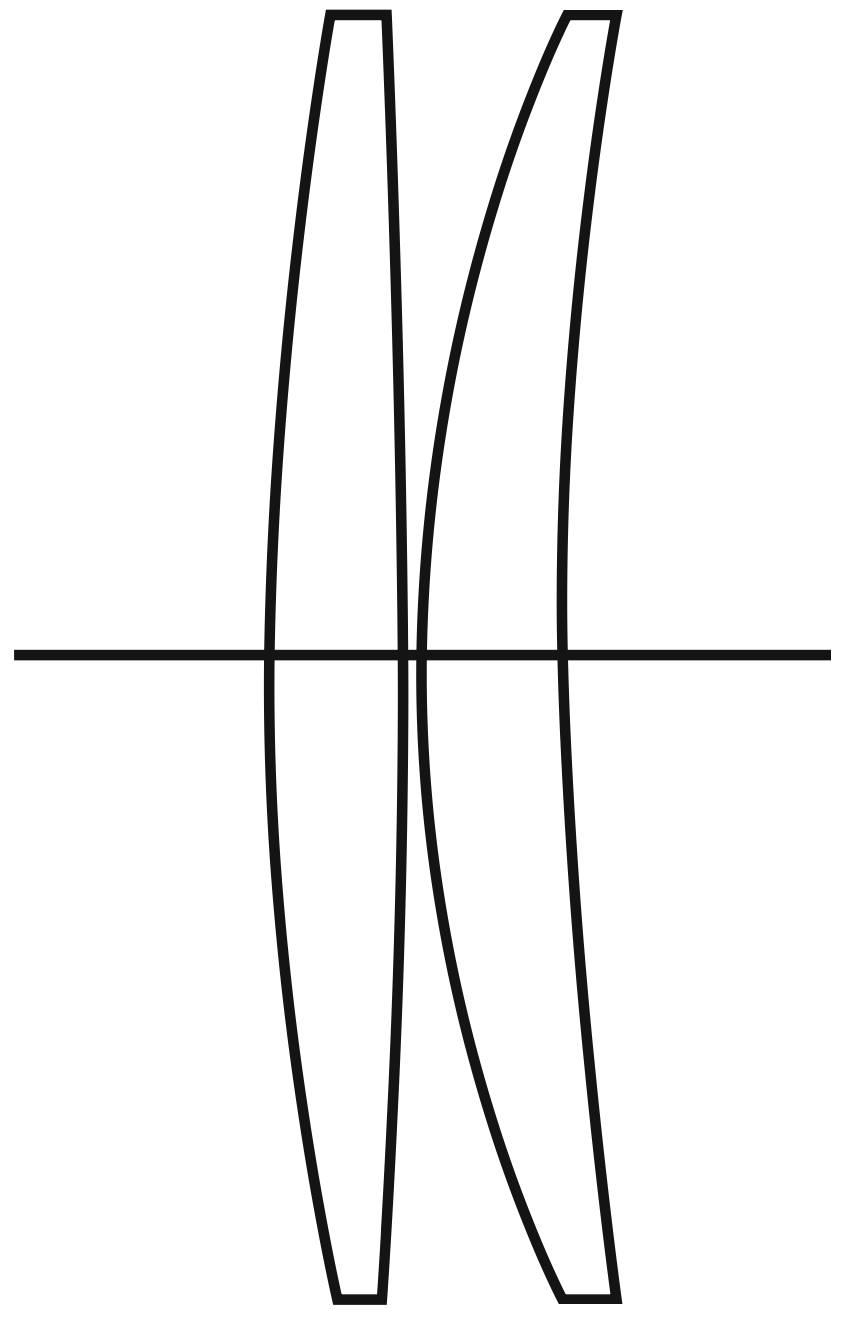
\includegraphics[width=\linewidth]{11} 
    \caption{График зависимости коллекторного тока $I_\text{к}$ от анодного
    напряжения $V_\text{a}$ для различных значений задерживающего
напряжения}
\label{fig:11}
\end{figure}

По графику на \fig{fig:11} определим энергию возбуждения первого
уровня атома гелия
\[
    E_1^\text{стат} = (30,7 \pm 0,9)\ \text{эВ}
\]







\section{Обсуждение результатов и выводы}
В работе было проведено измерение энергия первого уровня атом гелия в
динамическом и статическом режимах методом электронного возбуждения
\begin{equation*}
    \begin{aligned}
        E_1^\text{дин} &= (25,0 \pm 0,8)\ \text{эВ}\\
        E_1^\text{стат} &= (30,7 \pm 0,9)\ \text{эВ}
    \end{aligned}
\end{equation*}

Значение, полученное в динамическом режиме, в пределах погрешности
совпадает с табличным значением $E_1 = 24,6\
\text{эВ}$. (\url{https://physics.nist.gov/cgi-bin/ASD/ie.pl})












\end{document}
